\chapter{Testing Results}
\label{chapter:results}

%%%%%%%%%%%%%%%%%%%%%%%%% timing %%%%%
\section{Timing}

\begin{table}[h]
	\caption{The table shows the time in seconds to compute the different distances. Take note, that all metrics except the geodesic distance need to have the Laplacian eigenfunctions computed.}
	\begin{tabular}{c*{6}{|r}|}
		$|Vertices|$ &\begin{tabular}{@{}c@{}}Laplacian\\eigenfunctions\\/-values\end{tabular} & diffusion & \begin{tabular}{@{}c@{}}commute\\time\end{tabular}&
		biharmonic & \begin{tabular}{@{}c@{}}geodesic\\exact\end{tabular} & \begin{tabular}{@{}c@{}}geodesic\\Dijkstra\end{tabular}\\
		\hline
		1k  & 2.98   & 0.033 & 0.016 & 0.017 & 0.057  & 0.006 \\
		5k  & 12.46  & 0.122 & 0.064 & 0.070 & 0.481  & 0.014 \\
		10k & 30.35  & 0.283 & 0.157 & 0.169 & 1.449  & 0.036 \\
		20k & 65.08  & 0.487 & 0.268 & 0.288 & 3.632  & 0.063 \\
		50k & 206.58 & 1.193 & 0.655 & 0.705 & 12.123 & 0.149 \\
	\end{tabular}
	\label{tab:timing}
\end{table}

The average computation times to compute the distance from one point to all other points are condensed into table~\ref{tab:timing}.
We can see that the computation of the Laplacian eigenfunctions and eigenvalues takes the most time.
But after obtaining them, the computation time of the diffusion, the commute-time and the biharmonic distance are really short.
Since they all have the same basic structure, the small differences in speed are results of the different factors:
While the factor $\frac{1}{\lambda_i}$ of the commute-time distance is the fastest to compute, the additional square of the eigenvalue for the biharmonic distance makes it slightly slower.
The fact that the factor of the diffusion distance consists of an exponentiation and a product makes it the slowest one of those three.

One important thing to note here is that even though the computation of the Laplacian eigenfunctions and eigenvalues takes quite a bit of time, the result can be saved and reused every time the distance has to be computed.
So if we were to compute the distance between all points of the mesh (even with respecting the symmetry of the metric and therefore half the computations), the computation of the Laplacian based metrics is already faster then the exact geodesic distance on the mesh with 5000 vertices by an approximate factor of 4.

Even though the implementation of the geodesic is highly optimised, the exact geodesic distance is definitely the slowest metric to compute.
Here the propagation of the windows over all edges of the mesh comes into play.
In the paper \cite{surazhsky2005fast} it is stated, that the windows per edge increase exponentially and, since each new vertex is connected to the rest of the mesh by at least one edge, this means that the computation time has to increase at least at the same speed.
If you approximate the geodesic distance by the Dijkstra algorithm, the computation gets faster than every other metric but its quality decreases significantly.

\section{Sensitivity to noise, tessellation and deformation}

\subsection{Isolines}
Our first set of experiment results provides a visualisation of the different metrics on shapes from the SHREC 2010 dataset.
Similar to the experiments in \cite{lipman2010biharmonic}, we computed the distance from a single source vertex to all other vertices on the mesh, color coding it onto the mesh by using Phong shading, which results in a dark blue color for small distances and bright red colors for bigger values.
In addition to that we plotted white, equally spaced isolines onto the mesh to give a better visualisation of the properties of the chosen metric.

\paragraph{The geodesic distance}
\begin{figure}[h]
	\centering
	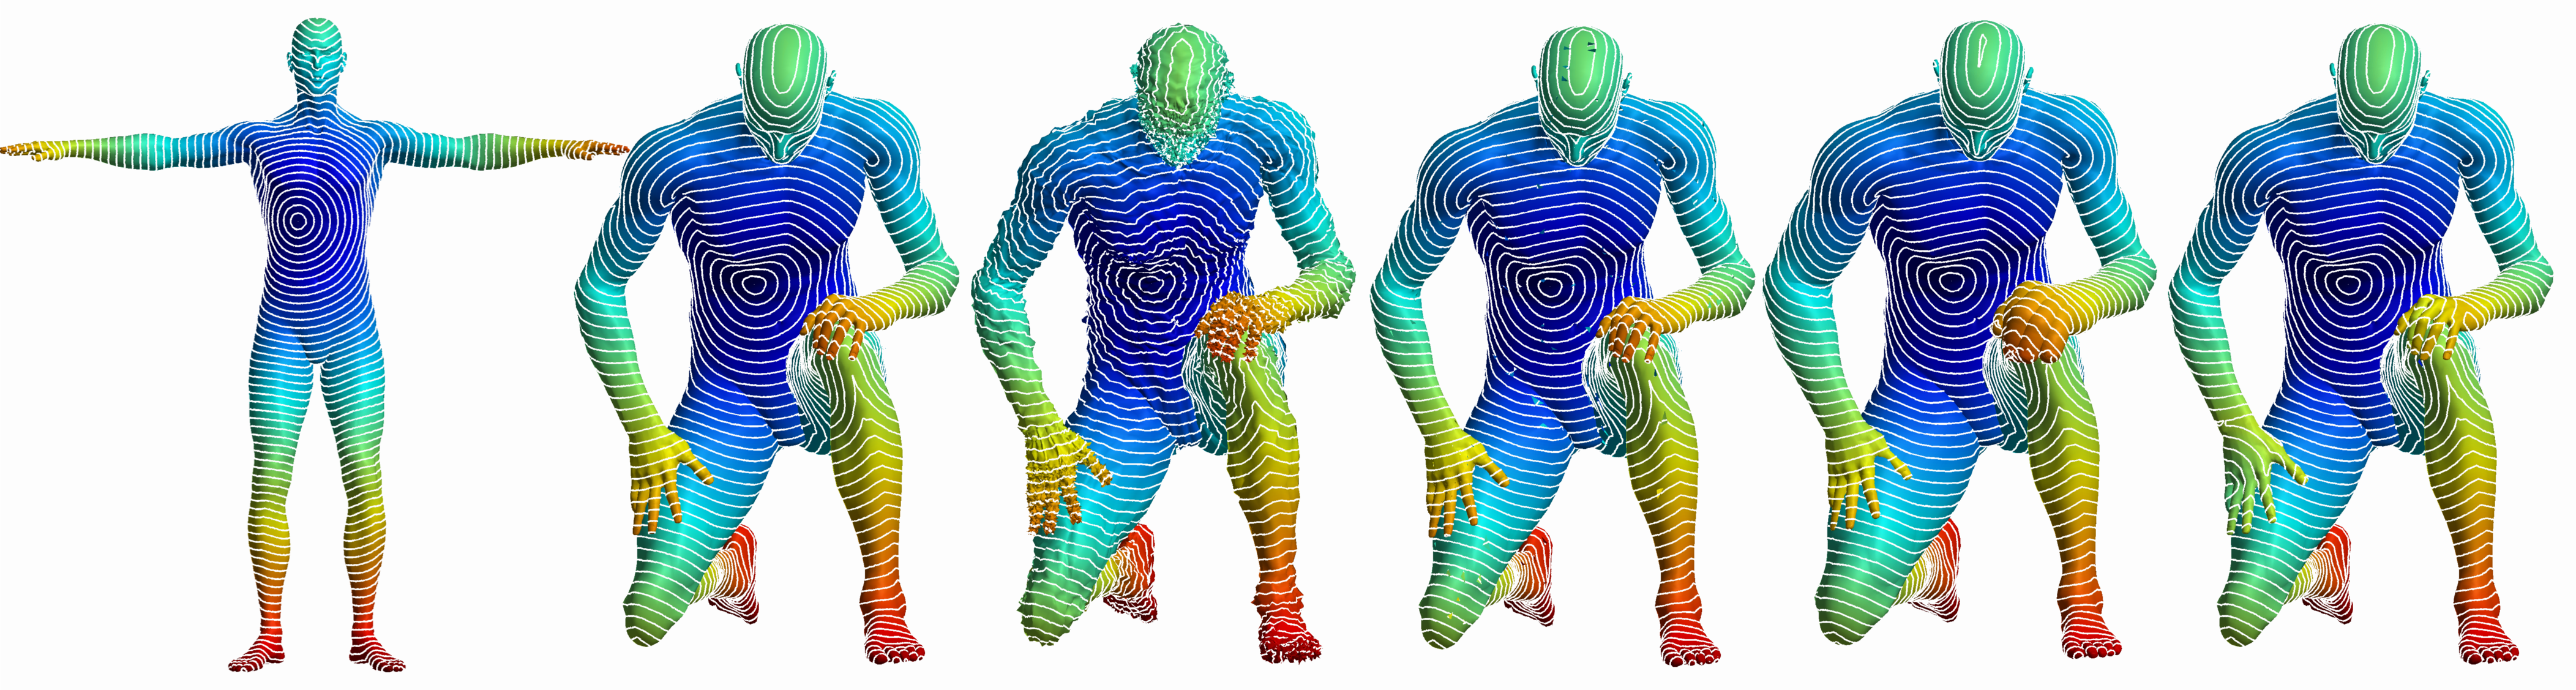
\includegraphics[width = \textwidth]{../results/geodesic_isolines}
	\caption{Comparison of the geodesic distance under different deformations of the mesh; from left to right: the null shape, isometry, noise, microholes, local scaling and topology changes.}
	\label{fig:geo_isolines}
\end{figure}
It is commonly known that the local properties of the geodesic distance are desirable.
As we can see on all meshes in figure~\ref{fig:geo_isolines}, the geodesic distance is isotropic and increases in a circular fashion, extending over the whole mesh.
There also lies its biggest flaw:
The geodesic distance is not globally shape-aware, which can be seen on the meshes as that the isolines run diagonal along the arms and legs.
This also means, that the shape of the isolines far from the source vertex depends on the exact placement of the starting point.
For example, would the source point lie somewhere on the left arm of the mesh, then the isolines would run perpendicular to the direction of the arm, forming small circles, instead of being distorted as they are in figure~\ref{fig:geo_isolines}.
Another point is that the geodesic distance is not smooth, as can be best seen on the locally scaled shapes left knee, where there is a big cusp.
In general, the geodesic distance results in cusps and ridges on the mesh, especially at the opposite side of the source vertex.
Furthermore, it is susceptible to topological changes or bigger holes in the mesh (which could not be tested):
On the corresponding mesh, the right hand is connected to the right thigh through a face, resulting in a significant change of the isolines (and therefore also the metric), since the shortest path through the upper leg is shorter than the geodesic distance before the change.
The isometric transformation from the null shape resulted in changed isolines on the legs, which again are a result of the missing global-shape awareness of the geodesic distance.
Apart from that, the geodesic distance is largely invariant to noise, small holes and local scalings.

\paragraph{The diffusion distance}
To begin with, the main difficulty with the diffusion distance is that it is not parameter-free.
It is possible to adjust the amount of global and local shape-awareness by choosing bigger or smaller $t$, but it is not possible to have both at the same time.
\begin{figure}[h]
	\centering
	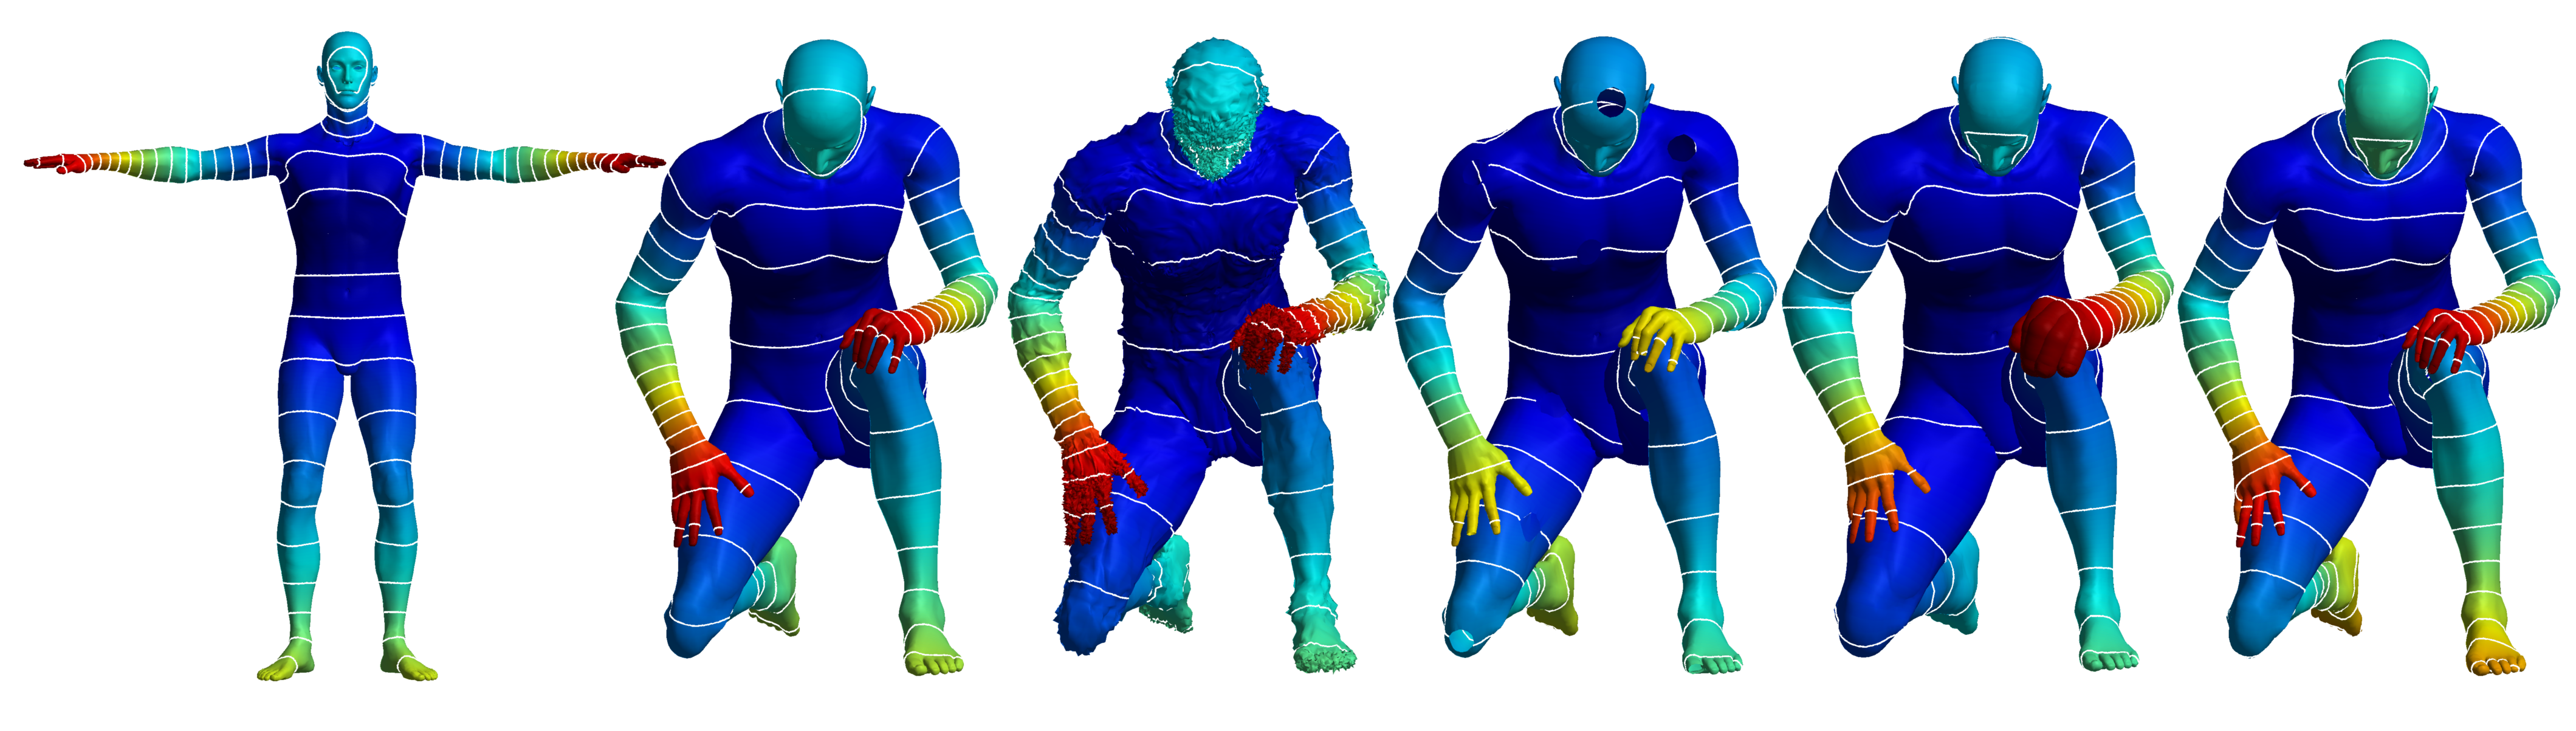
\includegraphics[width = \textwidth]{../results/diffusion_big_isolines}
	\caption{Comparison of the diffusion distance with $t = 1$ under different deformations of the mesh; from left to right: the null shape, isometry, noise, holes, local scaling and topology changes.}
	\label{fig:diffusion_b_isolines}
\end{figure}
We start by looking at the results of the diffusion distance with $t=1$.
The global shape-awareness of the diffusion distance is really dominant, resulting in isolines perpendicular to the central axis of protrusions as the arms or legs.
What can be seen close to the source point is that the global shape has an unwanted influence on the local distances, resulting in elliptic isolines close to the source vertex instead of circular ones.
This shows also, as with increasing $t$ the isolines close to the source vertex get closer and closer to being parallel instead of being circular.
As we already presumed the time parameter in this case favors the global properties, resulting in a not isotropic propagation close to the source.
Apart from that, the diffusion distance seem so almost invariant to the shown deformations of the shape.

\begin{figure}[h]
	\centering
	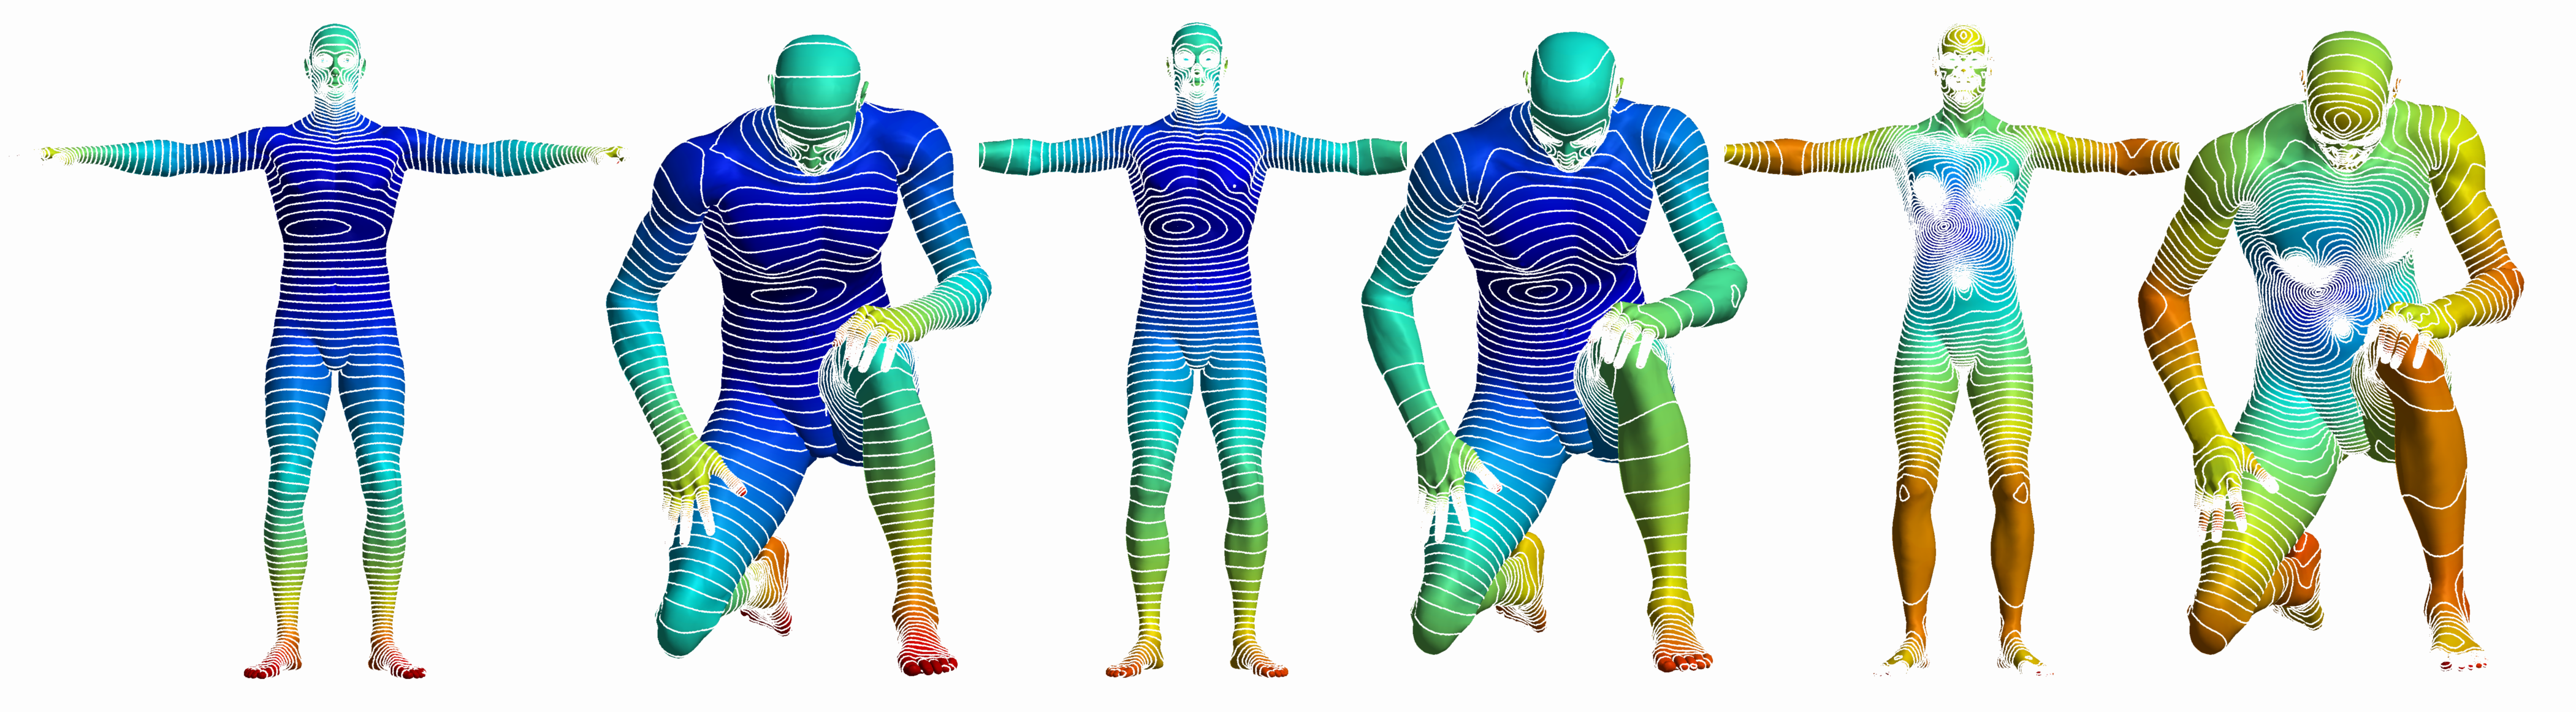
\includegraphics[width = \textwidth]{../results/diffusion_isolines_smaller_t}
	\caption{Comparison of the diffusion distance with $t = 0.1, 0.05, 0.01$ on the null shape and an isometric deformation; the value of $t$ decreases from left to right.}
	\label{fig:diffusion_s_isolines}
\end{figure}
In the second figure~\ref{fig:diffusion_s_isolines} we decided to show the behaviour of the diffusion distance with smaller $t$.
Even though the parameter with $t= 0.1$ is set to a relatively small value, it still has some good global properties, such as the isolines perpendicular to the central axis of protrusions as the arms or legs.
But on the other hand, the isolines close to the source vertex return to a more circular appearance.
This effect get more and more prominent, the smaller $t$ gets, revealing more and more detail close to the source vertex and loosing its global properties up to a degree, that the vertices far away from the source vertex are assigned near constant values, resulting in level sets with large areas.

\paragraph{The commute-time distance}
\begin{figure}[h]
	\centering
	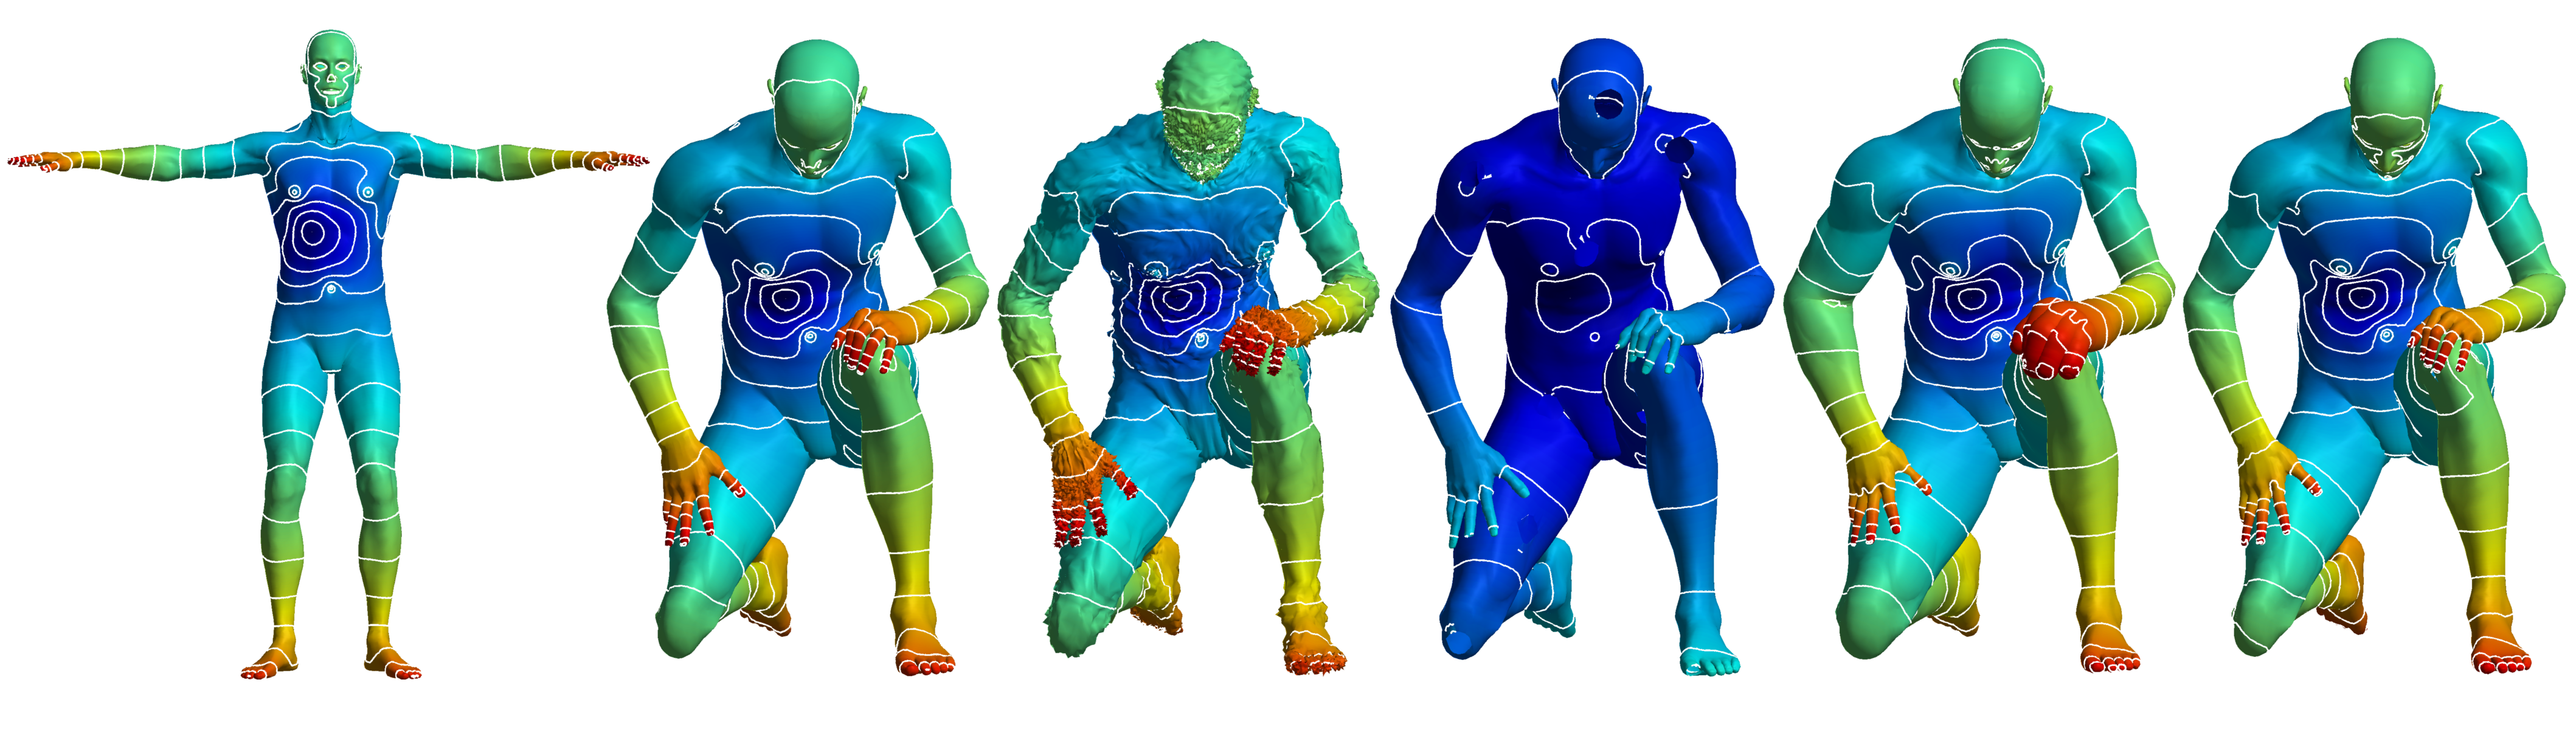
\includegraphics[width = \textwidth]{../results/commute_time_isolines}
	\caption{Comparison of the commute-time distance under different deformations of the mesh; from left to right: the null shape, isometry, noise, holes, local scaling and topology changes.}
	\label{fig:commute_time_isolines}
\end{figure}
The commute-time distance is, as mentioned in the subsection~\ref{subsection:commute}, the integral of the diffusion distance  over all $t$ and therefore being multi-scale without depending on a parameter.
As we can see in figure~\ref{fig:commute_time_isolines}, it obtained some of the diffusion distances properties:
The global shape-awareness has been preserved, as the isolines on the limbs are still vertical to their central axis, while the isolines close to the source point are close to circular.
But some of the influences of the diffusion distances result in unwanted behaviour, such as the local maxima at the belly button and around the belly.
These extrema in particular can be seen in figure~\ref{fig:diffusion_s_isolines} with really small $t$.
In addition to that the commute-time distance is not smooth, which can be seen by the isolines having crooks and cusps.
Concerning the different deformations, the commute-time distance seems to be only affected lightly by them, resulting in the isolines wandering a small distance up or down the limbs, but generally retaining their shape.
The only one which has large effect is the appearance of holes in the mesh.
For one, there are multiple local maxima at the edge of a hole, which is supplemented by the fact that we had to manually change the distance of the 60 (out of around 50k) vertices, which had the largest distance from the source point, to zero.
This minority of points had distance values up to double the maximal distance plotted in figure~\ref{fig:commute_time_isolines}.
So even though the isolines on the mesh with holes still resemble the others, the behaviour of the commute-time distance in this experiment is not desirable.

\paragraph{The biharmonic distance}
\begin{figure}[h]
	\centering
	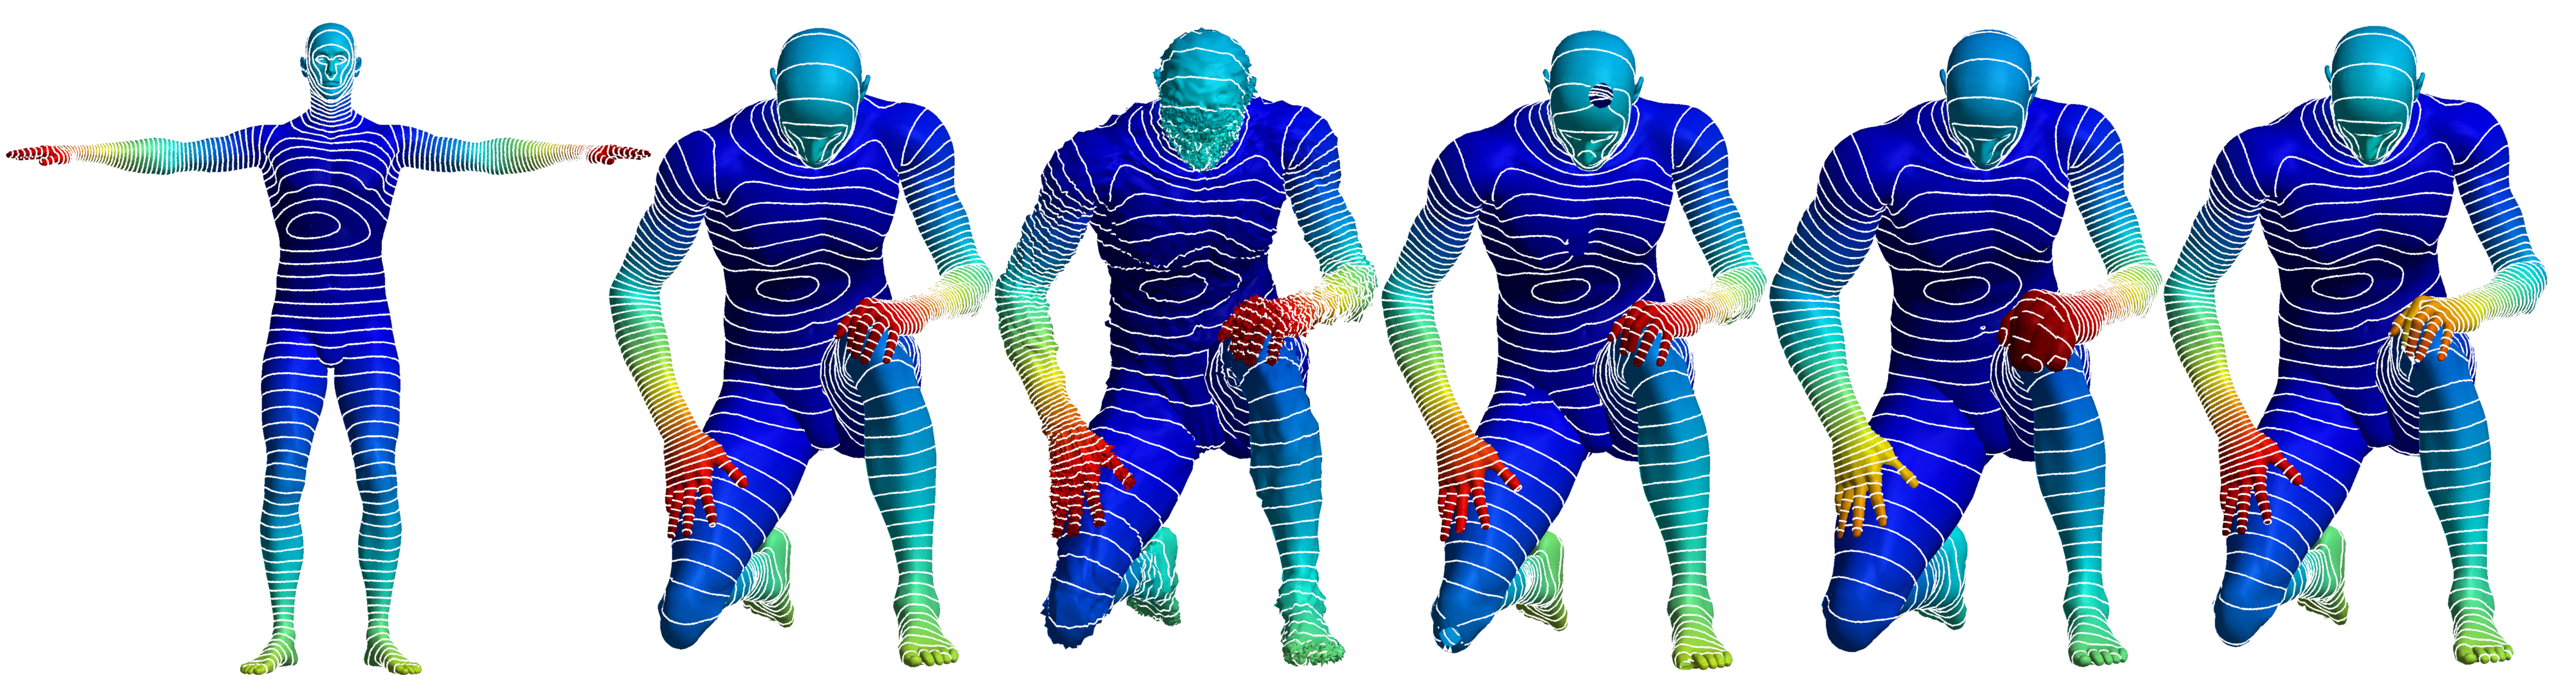
\includegraphics[width = \textwidth]{../results/biharmonic_isolines}
	\caption{Comparison of the biharmonic distance under different deformations of the mesh; from left to right: the null shape, isometry, noise, holes, local scaling and topology changes.}
	\label{fig:biharmonic_isolines}
\end{figure}
The last set of results, which shows the performance of the biharmonic distance, can be seen in excerpts in figure~\ref{fig:biharmonic_isolines}.
As it was designed to be, it is shape-aware and at the same time close to the geodesic distance in proximity of the source point.
This can be seen in the circular shape of the isolines close to the source, while the isolines follow the shape more and more, the farther they are from the source point.
Under the different deformations, the isolines and therefore the behaviour of the biharmonic metric is preserved in general.
Only on the arms undergoing  local scaling and topology changes the distance changes slightly, increasing the distance to one hand while decreasing the distance to the other.
But altogether, the biharmonic distance keeps its properties across all deformations.

\subsection{Farthest point sampling}
\begin{figure}[h]
	\centering
	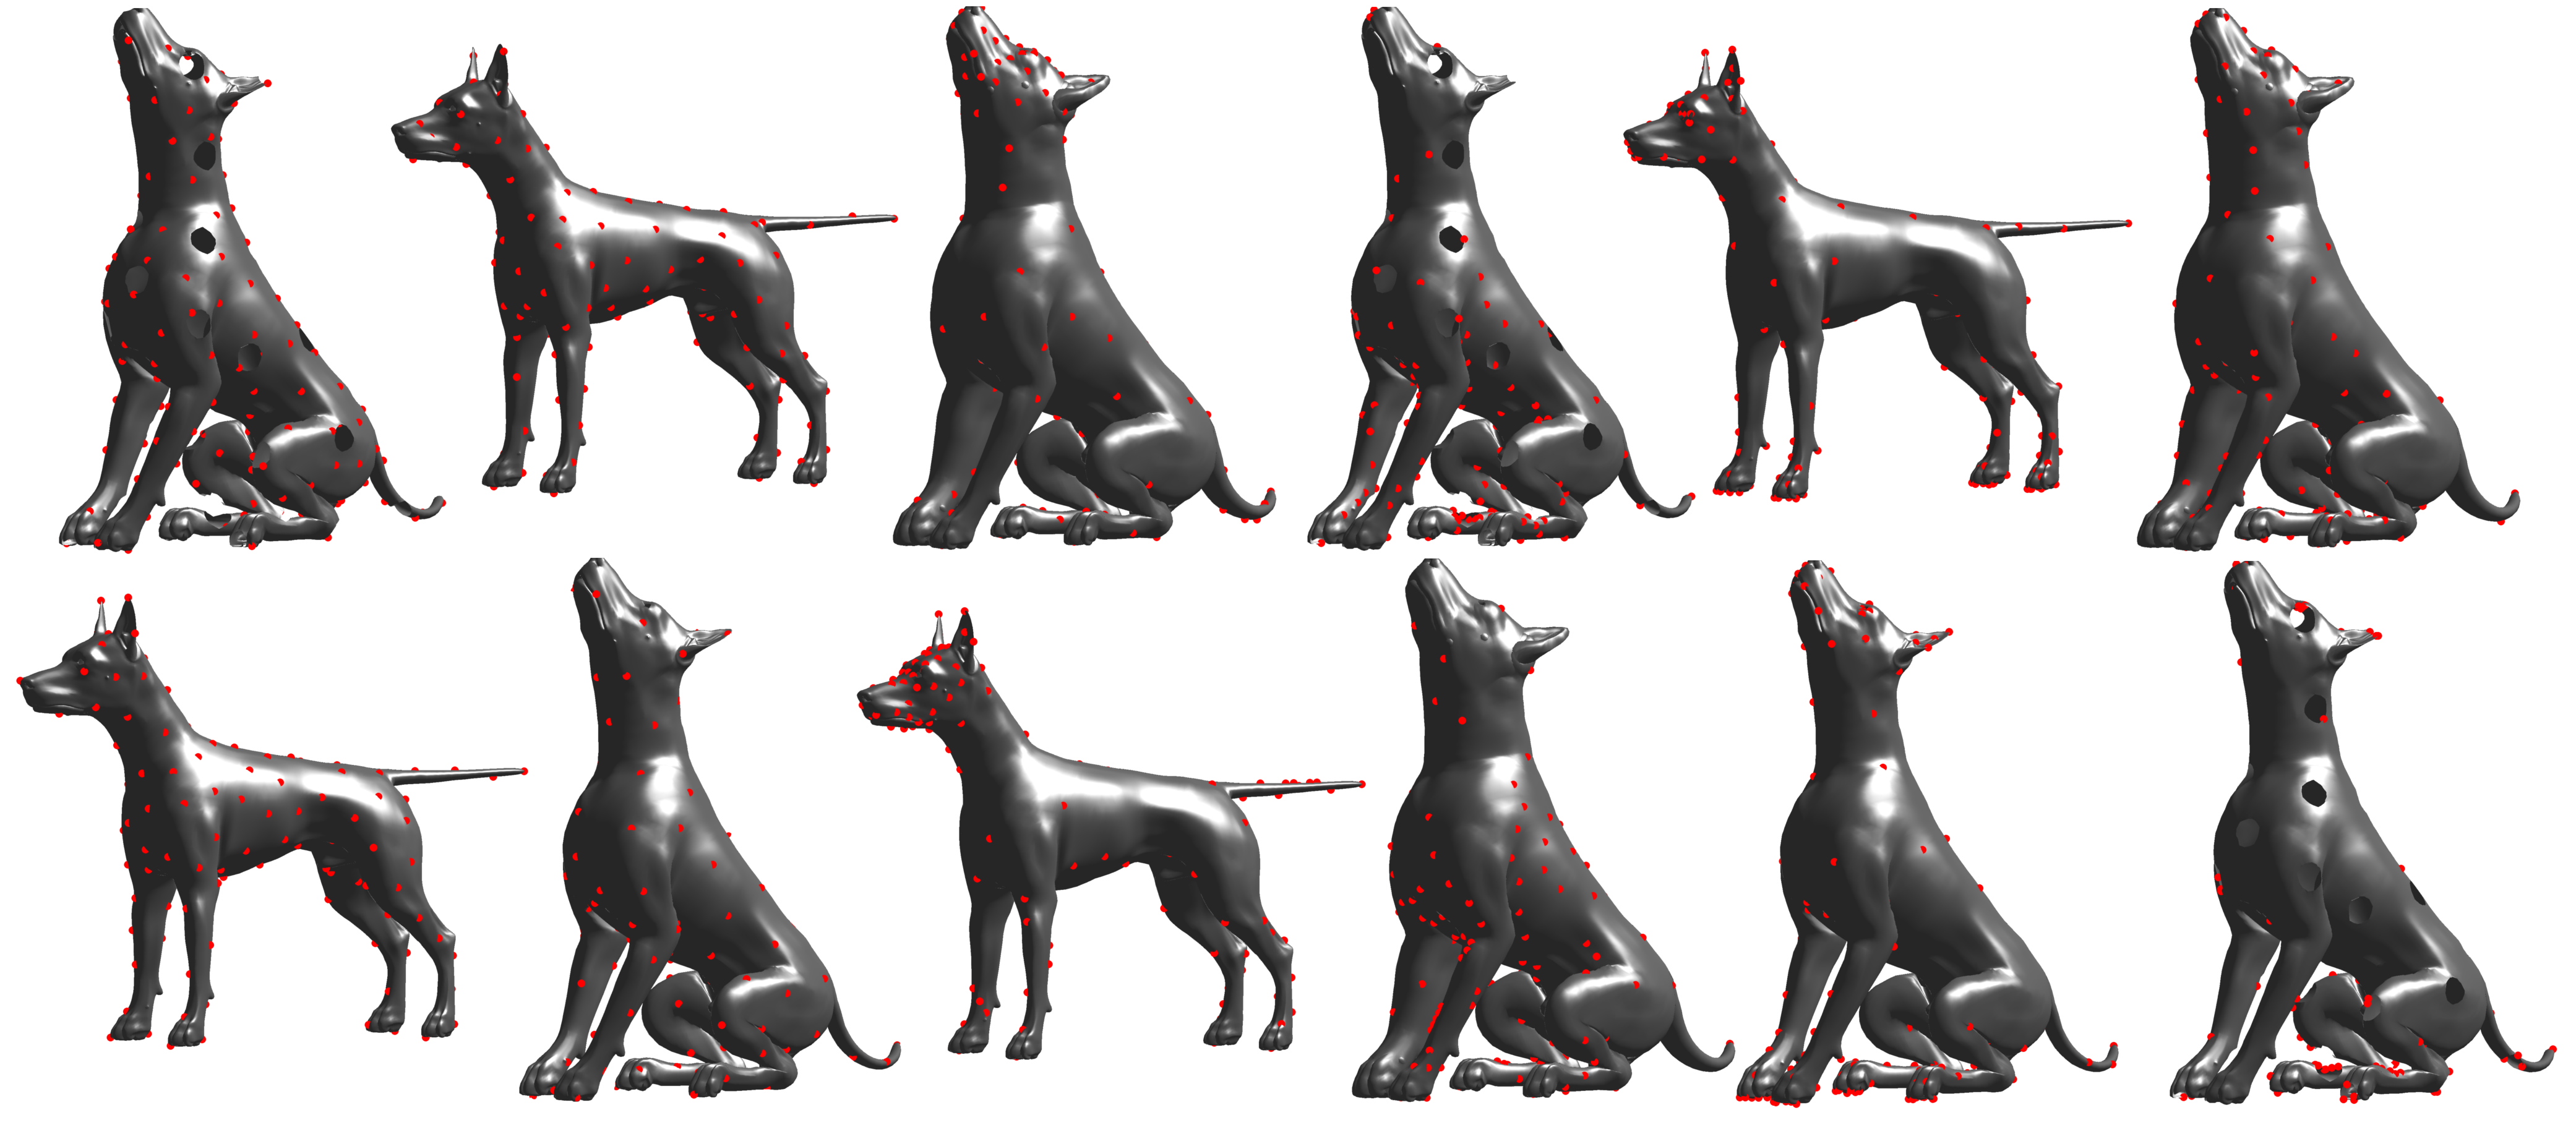
\includegraphics[width = \textwidth]{../results/fps_end}
	\caption{A selection of farthest point samplings of the different intrinsic metrics on shapes with holes, topology changes, local scale changes and the null shape; from left to right: Euclidean, geodesic, diffusion with $t=0.1$, diffusion with $t=1$, commute-time and biharmonic distance.}
	\label{fig:fps_end}
\end{figure}
The results of this experiment are quite straight forward:
Using the Euclidean distance results in the best, equally distributed set of vertices over the mesh, closely followed by the geodesic distance as can be seen in figure~\ref{fig:fps_end}.
The diffusion distance has an interesting effect, that depending on the parameter $t$ the points either cluster around the head of the dog or around the torso, leaving only a small number of vertices on the remaining body parts.
As has already happened during the plotting experiments, the commute-time distance intensifies the effects of small $t$, resulting in almost no vertices on the torso and clusters of points on the head and the legs of the dog.
While the FPS based on the biharmonic distance seems to be almost equally distributed on the upper part of the figure, the vertices of the lower part, showing the mesh with a number of holes, are concentrated on the legs and the head while covering almost nothing of the rest of the mesh.
This is probably for one a result of the difficulties of the metric to handle a mesh with holes and it can also be seen on the upper picture, that the biharmonic distance has a tendency to distribute the points with a bigger focus on the head and legs then on the torso.
Therefore the best results are being produced by the fastest and simplest metric of the set: the Euclidean distance.
Even though it is unusable in any of the other use cases of intrinsic metrics, like for example shape matching because of its missing invariance isometries, for the task of computing a farthest point sampling the Euclidean distance is the best.


\subsection{Error measurement}
We now review the results of our error computation with the different metrics.
As a reminder, the calculated values are the mean and maximal error between a mesh under a certain deformation and the null shape, divided by the maximum distance on the null mesh.
\begin{table}[h]
	\caption{The mean error of the distances, grouped by the type of deformation. The minimum value is underlined.}
	\begin{tabular}{@{}l*{8}{|r}|@{}}
		metric & isometry & \begin{tabular}{@{}c@{}}local\\scale\end{tabular} & scale & topology & noise & \begin{tabular}{@{}c@{}}shot\\noise\end{tabular} &
			\begin{tabular}{@{}c@{}}micro\\holes\end{tabular} & holes \\
		\hline
		geodesic		& .0232				& .0407				& .1580				& .0508				& .0218				& .0419				& .0417				& - \\
		diffusion t=0.1 & .0043				& .0310				& .0058				& .0408				& .0241				& .0044				& .0059				& .0434 \\
		diffusion t=1	& \underline{.0022} & .0320				& .0029				& .0223				& \underline{.0180} & \underline{.0018} & .0031				& .0528 \\
		commute-time	& .0034				& \underline{.0092} & .0037				& \underline{.0138} & .0309				& .0031				& .0035				& \underline{.0331} \\
		biharmonic		& .0049				& .0220				& \underline{.0016} & .0420				& .0625				& .0024				& \underline{.0017} & .0388 \\
	\end{tabular}
	\label{tab:mean}
\end{table}
As can be seen in table~\ref{tab:mean} there is no clear answer as to which metric is superior in regards to the metric distortion of the distance from one source point to all other points.
While it is obvious, that the geodesic and the diffusion distance with a small $t$ are no competition, the other metrics compete for the best mean errors.
The diffusion distance with $t=1$ is clearly the best for the categories isometry and noise, whereas the commute-time has the best mean errors for topology changes, changes in local scale and meshes with holes.
This can be tied to the alternate definition as the average time a random walker takes to go from one point to the other and return, which is not as strongly influenced by those deformations as the other metrics.
Finally, the biharmonic distance provides the smallest mean errors for scaled meshes and micro holes.
The bad performance of the geodesic and the more local version of the diffusion distance probably based on their bad shape-awareness.
Additionally, one can see that the geodesic distance is not scale-invariant, as the corresponding mean error is disproportionally high.

\begin{table}[h]
	\caption{The maximum error of the distances, grouped by the type of deformation. The minimum value is underlined.}
	\begin{tabular}{@{}l*{8}{|r}|@{}}
		metric & isometry & \begin{tabular}{@{}c@{}}local\\scale\end{tabular} & scale & topology & noise & \begin{tabular}{@{}c@{}}shot\\noise\end{tabular} &
			\begin{tabular}{@{}c@{}}micro\\holes\end{tabular} & holes \\
		\hline
		geodesic		& .0984				& .1554				& .4064				& .2227				& .1311				& .1567				& .1566				& - \\
		diffusion t=0.1 & .0258				& .2745				& .0347				& \underline{.0774} & .0728				& .0365				& .0346				& \underline{.2209} \\
		diffusion t=1	& .0217				& .1473				& .0301				& .2042				& \underline{.0685} & .0330				& .0302				& .4938 \\
		commute-time	& .0288				& .0899				& .0493				& .1598				& .1381				& .0487				& .0469				& .6374 \\
		biharmonic		& \underline{.0188} & \underline{.0648} & \underline{.0285} & .3226				& .1113				& \underline{.0275} & \underline{.0276} & .5229 \\
	\end{tabular}
	\label{tab:maxerror}
\end{table}
In our experiments measuring the maximum (relative) error, which can be seen in table~\ref{tab:maxerror}, the biharmonic distance had the best performance.
In five out of eight categories the biharmonic metric resulted in the smallest maximum error.
Only on meshes under topology changes, noise and with holes the diffusion distance was superior to the biharmonic distance.
Apart from that, note that the commute-time distance again showed inconsistent behaviour on meshes with holes, as it resulted in the smallest mean error but, similar to the isolines experiment, the biggest maximum error.

Altogether, the deformations can be separated into two classes, based on the performance of the metrics in regards to the  maximum error and independent of the specific metric:
The deformations resulting in relatively small maximum errors approximately ranging from two to 8 percent, namely isometry, local scale, scale, micro holes and shot noise and the more ``challenging'' deformations with maximum errors ranging from ten to 40 percent, namely noise, holes and topology.
The exact same partitioning of deformations can be extracted from table~\ref{tab:mean} by separating the deformations by the question, whether or not the majority of the metrics have a mean error below or above one percent, which means we can safely conclude that noise, holes and topology changes are the most challenging deformations of a mesh for all considered intrinsic metrics.
